% WARNINGS: 
%	    1. You must make sure that PDF output generated from this
%	       template is complete both when displayed with a viewer 
%	       (acroread, for example) and when printed on paper.
%	       LaTeX installations vary greatly and therefore it might 
%	       not be possible to get all proposals to come out 
%	       correctly with a single text page layout. 
%	       In some cases you will have to adjust the 
%	       \topmargin=-7mm command in the template to center the 
%	       text vertically in the page.  
\documentclass[12pt,a4paper]{article} 
\usepackage{times}
\usepackage{graphics,graphicx}
\usepackage[update,prepend]{epstopdf}
\usepackage[innercaption]{sidecap}
\usepackage{subcaption}
\usepackage{amssymb, amsmath}	       
\usepackage{xspace}				
\usepackage{natbibspacing, natbib}
\usepackage{aas_macros}
\usepackage{wrapfig}
\usepackage{floatrow}

\newcommand{\ncrit}{\mbox{$n_{\rm crit}$}\xspace}
\newcommand{\comol}{$^{12}$CO\xspace}
\newcommand{\Lsun}{\mbox{L$_{\odot}$}\xspace}
\newcommand{\LIR}{\mbox{$L_{\rm IR}$}\xspace}
\newcommand{\LFIR}{\mbox{$L_{\rm FIR}$}\xspace}
\newcommand{\rarr}{$\rightarrow$}
\newcommand{\aco}{\mbox{CO($J$=1\rarr0)}\xspace}
\newcommand{\bco}{\mbox{CO($J$=2\rarr1)}\xspace}
\newcommand{\cco}{\mbox{CO($J$=3\rarr2)}\xspace}
\newcommand{\eco}{\mbox{CO($J$=5\rarr4)}\xspace}
\newcommand{\rot}[3][HCN]{\mbox{#1($J$=#2\rarr#3)}\xspace} 
% default HCN; usage \rot[HCN]{3}{2} or \rot[\hcop]{4}{3}
\newcommand{\ahcn}{HCN($J$=1\rarr0)\xspace}
\newcommand{\dhcn}{HCN($J$=4\rarr3)\xspace}
\newcommand{\hcop}{HCO$^+$\xspace}
\newcommand{\ahcop}{\mbox{HCO$^+$($J$=1\rarr0)}}
\newcommand{\dhcop}{HCO$^+$($J$=4\rarr3)\xspace}
\newcommand{\Lp}[1][CO]{\mbox{$L^{\prime}_\textrm{\fontsize{8pt}{12pt}\selectfont{#1}}$}}
\newcommand{\LpU}{\mbox{K\,\,km\,\,s$^{-1}$\,\,pc$^2$}}
\newcommand{\kms}{km\,s$^{-1}$\xspace}
\newcommand{\pmOne}{\mbox{$^{-1}$}\xspace}
\newcommand{\Fig}[1]{Fig.~\ref{fig:#1}}
\newcommand{\Eq}[1]{Equation~\ref{eq:#1}}

%Compact BIB%%%%%%%%%%%%%%%%%%%%
\citestyle{aa}	
\bibliographystyle{apj_w_etal_3auth}

\usepackage{paralist}

\renewenvironment{thebibliography}[1]{%
%\section*{\refname}%
%  {\normalsize {\textbf{References:}}}
  \let\par\relax\let\newblock\relax%
  \inparaitem[{[}1{]}]}{\endinparaitem}
%%%%%%%%%%%%%%%%%%%%%%%%%%%%%


%%%%%%%%%%%%%%%%%%%%%%%%%%%%
%%%%%% Page dimensions %%%%%
%%%%%%	DO NOT CHANGE  %%%%%
%%%%%%%%%%%%%%%%%%%%%%%%%%%%

\textheight=247mm
\textwidth=180mm
\topmargin=-7mm
\oddsidemargin=-10mm
\evensidemargin=-10mm
\parindent 10pt

\renewcommand\floatpagefraction{.9}
\renewcommand\topfraction{.9}
\renewcommand\bottomfraction{.9}
\renewcommand\textfraction{.1}
% between fig
\setlength{\textfloatsep}{10pt plus 1.0pt minus2.0pt}
\setlength{\floatsep}{10pt plus 1.0pt minus 2.0pt}
\setlength{\intextsep}{10pt plus 1.0pt minus 2.0pt}
\setlength{\parskip}{0.01em}
\usepackage[small,tiny,compact]{titlesec}

\begin{document}
\pagestyle{plain}
\pagenumbering{arabic}
 
\begin{center}
{\large{\bf
{ 
Molecular gas dynamics and AGN/starburst mechanism in a
strongly-lensed wet merger: bridging the gap between local ULIRGs and high-z systems}
}}
\end{center}
\vspace{-0.545em}
\centerline{\normalsize{\bf PI: 
{T. K. Daisy Leung}}} 
%%%%%%%%%%%%%%%%%%%%%%%%%%%%%%%%%%
\vspace{0.1em} {\bf Missing link between mergers/ULIRGs and their high-z analogues} 
Ultraluminous infrared galaxies (ULIRGs: \LIR$\geq$10$^{12}$\Lsun) have been
regarded as analogues of high-redshift (z) starbursts given the
similarities in their interstellar medium (ISM; e.g. \LIR/\Lp).
As such, detailed studies 
of ULIRGs are important 
to gain more detailed insight into the early universe and in studies of galaxy evolution over cosmic time.
While mergers are believed to play an important role in giving rise to these dusty galaxies
(e.g. Sanders \& Mirabel 1996), merger-induced effects on the physical mechanisms and chemistry 
that drive the 
%intense 
starburst (SB) and active galactic nucleus (AGN) activities on small scales are still unclear.
Thus characterizing the properties of the molecular gas that fuels star-formation (SF) and AGN is
crucial to understand the interplay between AGN and SB
and their relation to the ISM properties of galaxies across cosmic time.

While the ISM in local ULIRGs has been studied in great detail,
forming a rich inventory of molecular transitions that serves as the template for 
studying high-z galaxies 
\citep[e.g.][]{Rangwala15a}, a wide knowledge gap persists
between $z$=0 and the epoch when most stars are formed in the universe ($z$$\sim$2). 
Hence, understanding galaxy populations at an epoch when
the build-up of stellar mass 
is steeply rising is critical and we here aim to bridge this gap by testifying
correlations and properties found locally out to high redshift by observing the 
dynamical structure and properties of the ISM of
the quadruply lensed galaxy RXJ1131-1231 and its dust-obscured 
companion at $z_{\rm CO}$$\sim$0.65 (\Fig{HST}).

\noindent {\bf Molecular gas in AGN/SB} 
Owing to the high molecular gas fractions in ULIRGs,
% and their high-z analogues, 
their extreme SFRs are a natural consequence of either gas is being converted into stars
more efficiently and/or their molecular gas content. Fragmentation
of giant star-forming clumps and turbulent conditions are also expected 
from gravitational instability of these gas-rich bodies. 
In fact, studies of the ISM kinematics at $z$=1-2 find clumps of size scale
 $\sim$few kpc \citep{Swinbank12a, Swinbank12b}. 
Resolving the gas dynamics on hundred pc scales is therefore an important first step
to understanding the mechanisms and physical processes taking
place on different scales and how the ISM physical conditions 
are related to the SB in ULIRGs at this epoch. %(when the SFR density is steeply rising).

While \comol emission traces the total molecular distribution and dynamics,
high-dipole moment molecules such as HCN and \hcop are expected to trace the 
%properties of the 
denser, actively star-forming gas. Indeed, a tight correlation between \ahcn and \LIR 
(proxy for SFR) has been found in nearby galaxies and local giant molecular 
clouds (GMC; \citealt[hereafter GS04]{Gao04a}; \citealt{Wu05}), 
suggesting HCN is a faithful tracer of the star-forming dense gas.
% and that the origin can be attributed to the fundamental units of star formation. 
However, \dhcn observations of (U)LIRGs have revealed a wide range of
excitation conditions 
%for their dense gas phase 
that may render the ground state transition of 
HCN and \hcop poor proxies of the dense gas mass \citep[hereafter P07]{Papadopoulos07a}.
In this light, higher-$J$ transitions (e.g. $J$=4\rarr3) 
% are necessary to scrutinize the reliability of using the ground state 
have been suggested to be better probes
% dense gas mass tracers since the mid-$J$ transitions
since they trace the much denser gas (n$\gtrsim$10$^5-$10$^7$ cm$^{-3}$) that is 
thought to be the immediate fuel for SF in turbulent GMCs \citep{Shirley03a, KM05}. 
This has been supported by the linear correlations found in 
\LIR-\Lp[\dhcn] and \LIR-\Lp[\dhcop] \citep[]{Zhang14a}.
Since the 
ground state lines are redshifted to frequencies beyond the spectral coverage of ALMA
at $z$$>$0.06, it is also necessary to establish diagnostics using these mid-$J$ lines to 
study distant galaxies.
Additionally, due to the difference in abundances and excitation conditions of HCN and \hcop
in star-forming versus AGN regions, the line 
% ratios \ahcn/HCO$^+$($J$=1\rarr0) \citep{Kohno05a, Imanishi10, Izumi13a} and
ratio \dhcn/\dhcop \citep{Imanishi14a, GB14a, Viti14a} have been 
proposed as
%  diagnostic tools 
a diagnostic tool to reveal deeply buried AGNs at the cores of ULIRGs \citep{Izumi16a, Imanishi16a}.
% separate emission originating from AGN and SB
% Recent studies have
% extended this diagnostic to using the J=4\rarr3 transitions 
%\citep{Imanishi14a, GB14a, Viti14a}, 
% where an elevated line ratio is seen in AGNs, suggesting
% it can be used to reveal deeply buried AGNs at the cores of ULIRGs \citep{Izumi16a, Imanishi16a}.

Prior to ALMA, studies of dense gas were largely limited to the local universe ($z$$\lesssim$0.1) 
with only five detections
%IR-luminous lensed galaxies detected 
at $z$$\gtrsim$0.3
(e.g. \citealt{Riechers07a, Riechers10a, Wagg05a, Gao07a}).
Moreover, none of these 
spatially resolve the emission, rendering it difficult 
to draw more detailed conclusions on the dense gas properties of galaxies at high z. 
Even with ALMA, such studies will remain challenging, but by combining 
the magnification provided by gravitational lensing with the exceptional spatial resolution and sensitivity of ALMA, 
studies
of dense molecular gas in distant galaxies are now possible, as proposed here.

%%%%%%%%%%%%%%%%%%%%%%%%%%%%%%%%%% 
% \section*{Science Target RXJ 1131-1231: a demonstrative case at high-z}
% \vspace{-0.25em}
\noindent {\bf Science Target RXJ 1131-1231: a demonstrative case at high-z}
\vspace{-0.6em}
%\begin{figure}[!tbhp]
%\centering
%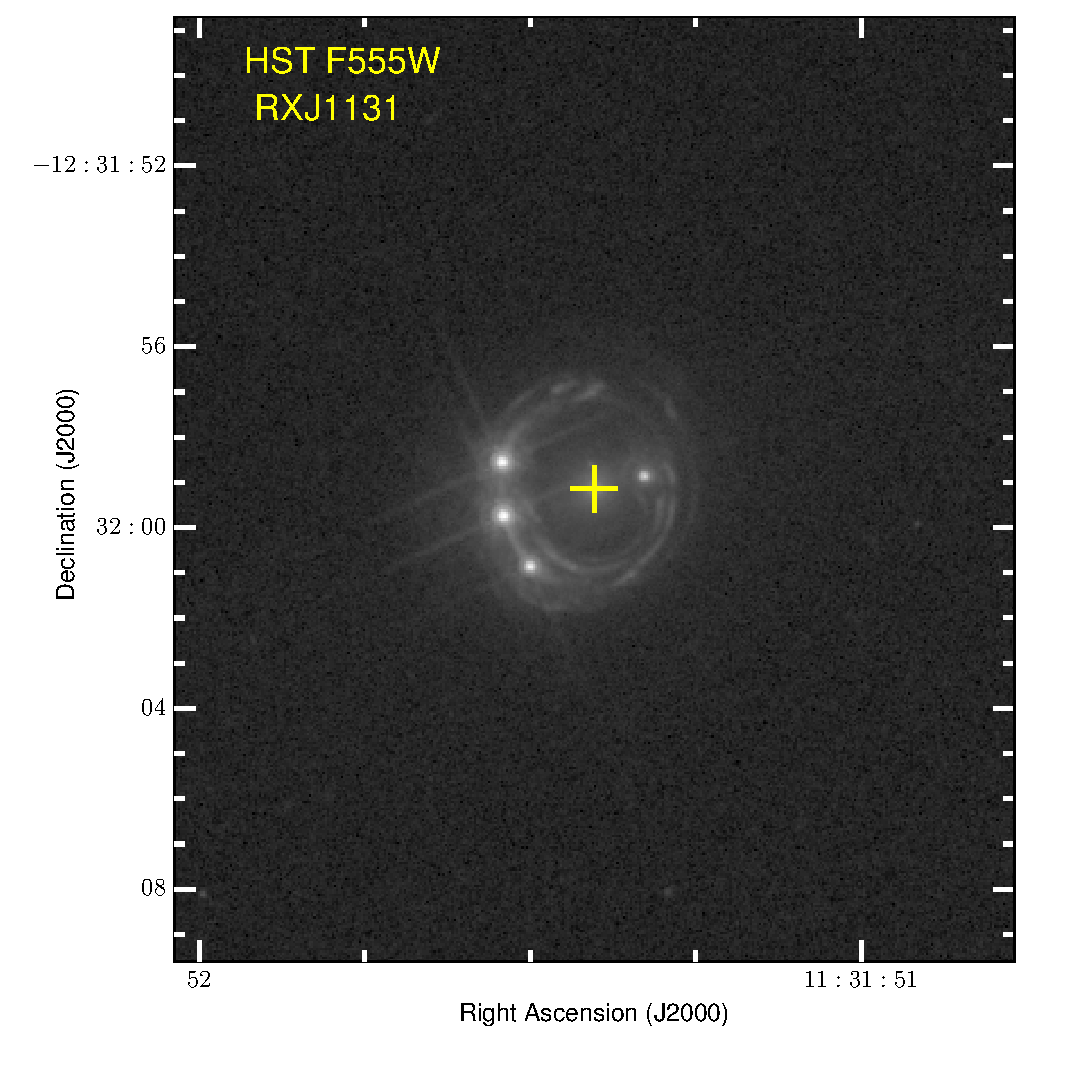
\includegraphics[trim= 10 20 15 0, clip, scale=0.3]{Fig/F555W} % &
%\hspace{-0.5em}
%\includegraphics[trim= 10 0 0 0, clip, scale=0.37]{Fig/Manipulate_figsCROP}
%\vspace{-1em}
%\caption{ \fontsize{10pt}{12pt}\selectfont 
%{
%\textbf{Stellar light distribution in the AGN host galaxy of RXJ 1131-1231 and its reconstructed source plane
%morphology}
%{\em Left:} The rest-frame UV emission (tracing recent star formation) 
%is lensed into an almost complete Einstein ring with diameter $\sim$ 3.8". 
%{\em Right:} Lens modeling of the optical emission identifies complex structure in the host galaxy and
%an optically faint companion (white; \citealt{Claeskens06a}), 
%which we have recently confirmed by modeling \bco emission detected with NOEMA
%(\Fig{combine}; Leung \& Riechers, in prep.). 
%We here propose to study
%the ISM conditions in this AGN-starburst composite system and offers an unparalleled
%view into the early universe, with finer
%detail than otherwise possible with current facilities. 
%}
%\label{fig:HST}}
%\end{figure}

\begin{figure}[!tbhp]
\centering
\hspace{-0.85em}
\floatbox[{\capbeside\thisfloatsetup{capbesideposition={right,center},capbesidewidth=0.445\textwidth}}]{figure}[\FBwidth]
{
\vspace*{-0.55em}
\hspace{-0.435em}
\raggedleft
\caption{ \fontsize{10pt}{12pt}\selectfont 
{\textbf{Stellar light distribution in the AGN host galaxy of RXJ 1131-1231 and its reconstructed source plane
morphology}
{\em Left:} The rest-frame UV emission (tracing recent star formation) 
is lensed into an almost complete Einstein ring with diameter $\sim$3.8". 
{\em Right:} Lens modeling of the optical emission identifies complex structures in the host galaxy and
an optically faint companion (white; \citealt{Claeskens06a}), 
which we have recently confirmed by modeling \bco emission detected with NOEMA
(\Fig{combine}; Leung \& Riechers, in prep.). 
We here propose to study
the ISM conditions in this AGN-starburst merger with finer
detail than otherwise possible with current facilities. 
}
\label{fig:HST}}}
{\hspace{-1em}
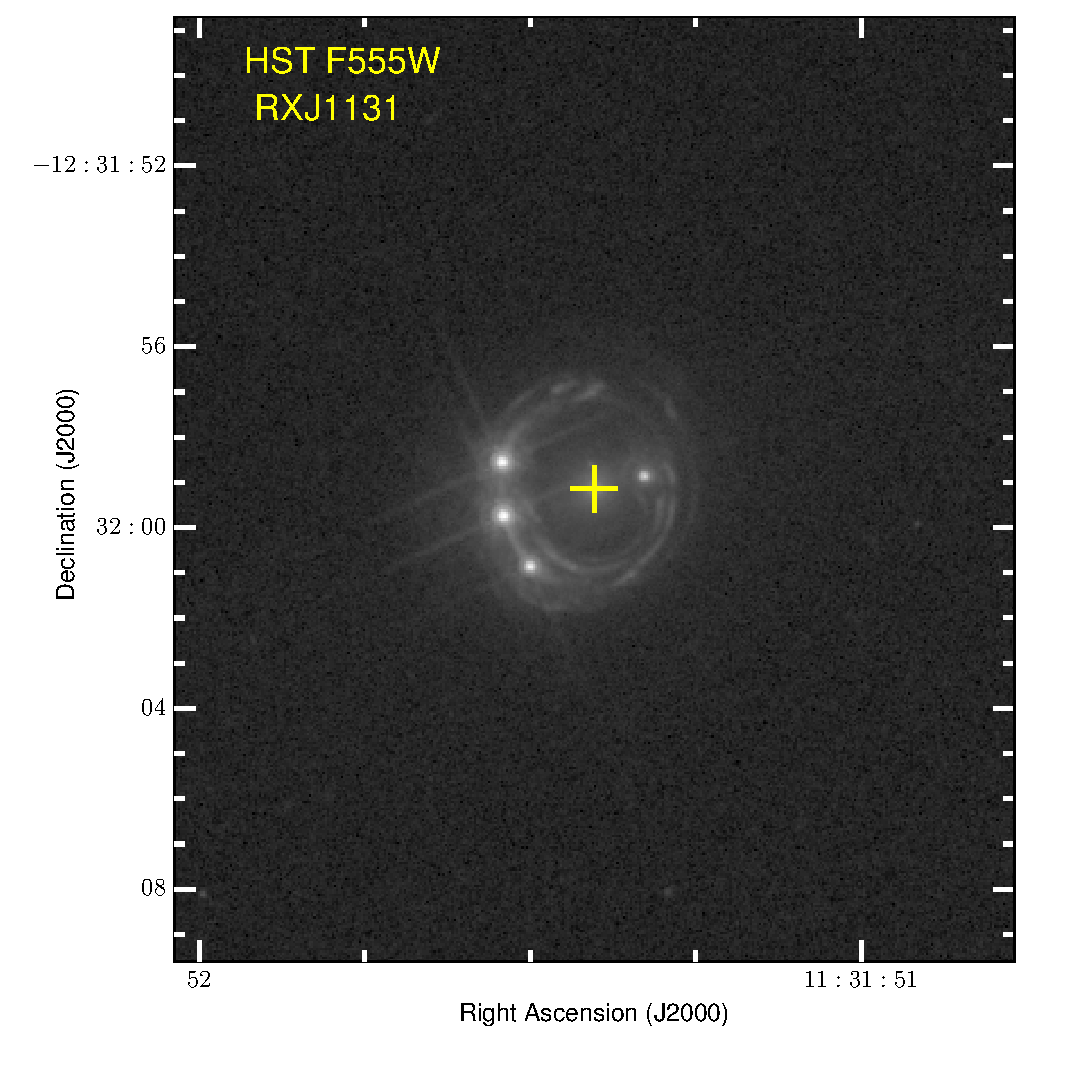
\includegraphics[trim= 10 20 15 0, clip, scale=0.28]{Fig/F555W}
\hspace{-1.5em}
\includegraphics[trim= 10 0 0 0, clip, scale=0.3]{Fig/Manipulate_figsCROP}
\vspace{-1.0em}
\hspace{-0.5em}
}
\end{figure}
\vspace{-0.8em}
RXJ 1131-1231 is a quadruply imaged AGN with its host galaxy lensed 
into a partial Einstein ring (\Fig{HST}). 
HST observations (rest-frame UV) have revealed distinct emission 
from recent star formation (lensing arcs) and from the AGN (bright knots) in the background galaxy \citep{Sluse03a},
demonstrating the great potential for probing its
ISM conditions in detail. Lens modeling carried out on optical images shows
that the AGN resides in a star-forming region of size $\sim$1 kpc
% $\sim$0.15" (without lensing magnification)
in its host galaxy, which itself is 7 kpc across, % $\sim$ 1 " (without lensing)
and made it possible to identify
seven distinct structures in the source plane (\Fig{HST}). Remarkably, emission 
%originating 
from 
a spatially offset region ($\sim$2.4 kpc away from the AGN host galaxy) has been identified and found 
to be $\sim$700 pc in size \citep{Brewer08a}, indicating a 
%nearby 
companion galaxy. 
We have recently confirmed that both galaxies are at the same redshift by detecting their 
\rot[CO]{2}{1} emission and lens-modeling their gas distribution 
in velocity space (\Fig{combine}f), and verified
that the both are gas-rich (Leung \& Riechers, in prep.). 
Our SED modeling of the dust continuum emission up to 250\,$\mu$m finds $L_{\rm IR}\sim6\times$10$^{12}$\Lsun 
(corrected for lensing). Hence, this target is a gas-rich ULIRG merger at $z$$\sim$0.7 caught in the act. 

%%%%%%%%%%%%%%%%%%%%%%%%%%%%%%%%%%
% \section*{Proposed Observations and Immediate Objectives}
% \vspace{-0.25em}
\noindent {\bf Proposed Observations and Science Goals}
We here propose to map (1): \eco at 0.15" resolution ($\sim$500pc at $z$$\sim$0.7 in the source plane) and 
(2): \dhcn and \dhcop emission and the underlying continuum at 0.7" resolution (2.5 kpc in the source plane).
The continuum traces the dust emission, 
providing better constraints on the the gas-to-dust ratio, dust temperature(s), dust mass,
and its spatial extent (and thus the surface density of the SFR).
%($\Sigma_{\rm SFR}$).
These quantities are key to investigate how the ISM % conditions 
vary as galaxies evolve across cosmic time.
In conjunction with the large set of ancillary data from
rest-frame UV to radio wavelength and our recent observations of \bco and \rot[CO]{3}{2}, our
proposed observations are designed to investigate 
% carry a detailed investigation of 
the gas-rich merger in aspects listed as follows.

\underline{\bf Dynamics and kinematics:}
Our recently obtained \bco data shows an asymmetric double-horned line profile (\Fig{combine}a). Given
the 1$^{\rm st}$ moment map observed and the velocity gradient
across the source plane in our model (\Fig{combine}d \& \ref{fig:combine}f), this is indicative of
a kinematically ordered %(reminiscent of a rotating disk) 
galaxy, but its emission has been lensed differentially. 
Limited by the spatial resolution of this data, it is not possible to infer the true 
kinematics due to beam smearing.
Furthermore, the unusually high velocity dispersion 
$\gtrsim$400\kms at the central region (\Fig{combine}e) hints at 
perturbations from the AGN and/or
internal turbulence
% motion 
due to interactions with the companion
and/or instability due to the huge gas reservoir.
Thus higher-resolution \eco imaging, as proposed here, is needed
to distinguish 
between a merger-driven and a turbulent clumpy disk starburst, 

The requested resolution (0.15") for \eco is critical
as it allows us to obtain a detailed
dynamical lens model of the system, probing at sub-kpc scale % probe down to 0.15" <-> 500 pc
(typical size scale of high-z GMCs), which enables us 
to compare the spatial distributions of star-forming gas clumps 
with recent star-formation (from HST).
Such comparisons are the key to understand different processes
that regulate the star-formation/SB
in ULIRGs/mergers and examine how they differ from other galaxy populations.
% kinematics
We will also measure the linewidths of the very dense gas (traced by HCN and \hcop), 
the excited gas (traced by \eco), and the more-extended, less-perturbed 
molecular gas (traced by low-$J$ CO) at various regions within the AGN host galaxy 
to constrain the kinematics and relative mass-fractions of different gas phases, 
which are indications of the evolutionary stage of a galaxy.

\underline{\bf Line ratios and the AGN/SB diagnostic:}
Aided by lensing, we will be able obtain kinematical information on spatial 
scales smaller than the beam, as seen in our \bco data (\Fig{combine}c, d), thereby
% and thus recover structural details and kinematics in finer detail than otherwise possible
enabling us to probe the physical properties of
the inner molecular disk near the AGN. 
% At the proposed resolution, we will be able to distinguish the \dhcn and \dhcop
% emission originating from the AGN host galaxy (and within) and from its companion.
Recent studies find that the \dhcn/\dhcop line ratio is expected to be enhanced 
in the circumnuclear disk (CND) near an AGN and falls off with distance from the CND
\citep{GB14a,Imanishi16a}. At the proposed resolution, we will 
resolve the line emission originating near the AGN and that from the spatially extended 
SB regions ($>$kpc scale) in the host galaxy, and by measuring spatial variations in 
this line ratio, we will assess its utility 
as an AGN/SB diagnostic (\Fig{AGNSB}) at high redshift.
Since the HCN vibrational line (v$_2$=1) falls within the targeted frequency range, 
we will use it to independently constrain the radiation properties of the AGN environment, 
given that this line is excited by infrared pumping and that the radiation
field associated with the AGN is the cause of the elevated \dhcn/\dhcop
\citep{Sakamoto10a,Imanishi13a}.
The proposed spatial resolution is also necessary for
a detailed lens modeling of each emission line, enabling measurements of reliable line 
ratios, without significant uncertainties due to differential lensing.
Such measurements are vital to reveal how galaxy interactions drive gas into 
inner disks to initiate SB/AGN activities and how the ISM differ from 
normal star-forming galaxies.

\begin{figure*}[!tbph]
\vspace{-0.8em}
\hspace{-0.65em}
\centering
\floatbox[{\capbeside\thisfloatsetup{capbesideposition={right,center},capbesidewidth=0.565\textwidth}}]{figure}[\FBwidth]
{\includegraphics[trim=15 0 5 10, clip, width=0.385\textwidth]{Fig/izumi15}}
{
\hspace{-1.25em}
\vspace{-1.15em}
\caption{ \fontsize{10pt}{12pt}\selectfont {\textbf{\dhcn/\dhcop as AGN/SB diagnostic}
Difference in line ratios between local AGNs, SBs, and (U)LIRGs with buried AGNs suggest
that \dhcn/\dhcop can be used as a diagnostic tool to reveal the dominant power source within the
beam, where an elevated line ratio is seen in AGN and circumnuclear regions relative to SB regions/galaxies.
Such diagnostic depends heavily on the spatial resolution, as demonstrated by the
measurements taken with APEX (empty circle) and ALMA (filled circles) in NGC1068.
We here propose to spatially resolve this line ratio within the AGN host galaxy and obtain
measurements near the AGN and the extended SB regions to investigate spatial variations 
in order to assess its utility as a AGN/SB diagnostic at high redshift.
(Figure taken from \citealt{Izumi16a})}
\label{fig:AGNSB}}
}
\vspace{-0.905em}
\end{figure*}

% 
% mounting supporting evidence for such elevated
% HCN emission at the centers of local Seyfert galaxies has been accumulated (e.g., Kohno
% et al. 2001; Imanishi et al. 2006; Krips et al. 2008), giving an empirical AGN diagnostic.
%
%mounting evidence that HCN lines can be
%overluminous with respect to the lines of other dense molecular
%gas tracers, like HCO+, in the circumnuclear disks of
%Seyferts (Kohno et al. 2001; Usero et al. 2004; Kohno 2005).
%A significant percentage of luminous and ultraluminous infrared
%galaxies (LIRGs and ULIRGs) has also been reported
%to show high HCN/HCO+ intensity ratios (Graci�-Carpio et al.
%2006; Imanishi et al. 2006, 2007).
% 
%  More recently, spatially resolved ALMA observations
% of HCN(4-3) and HCO+(4-3) at the CND of NGC 1068 at a ?50 pc resolution reveal
% that the HCN(4-3)/HCO+(4-3) line ratios are indeed highly elevated at the CND but
% not significantly at the very position of the active nucleus (Garc??a-Burillo et al. 2014;
% Viti et al. 2014). This indicates that HCN enhancement is not simply caused by X-ray
% irradiation. Recent HCN(4-3)/HCO+(4-3) measurements of the high-luminosity
% type-1 AGN NGC 7469 (Izumi et al. 2015a) with LX = 2 � 1043 erg s?1
% suggest that the
% degree of HCN enhancement is not very different from that in NGC 1097 (Izumi et al.
% 2013), a much lower luminosity type-1 AGN (LX = 7�1040 erg s?1
% ), also adding further
% evidence against the XDR origin of enhanced HCN in AGNs (see also Mart??n et al. 2015).
% 
% XDR versus PDRs
Since \eco is excited in higher temperature than the HCN and \hcop lines (e.g. in 
X-ray dominated regions (XDRs) near an AGN), 
variations in HCN/CO will allow us to constrain the spatial extent of photon-dominated regions
 (PDRs from SBs) and XDRs.
% physical properties
In addition, we will measure spatially resolved line ratios of HCN/CO and \hcop/CO within the AGN host galaxy
as proxies of its very dense (cores; $\sim$10$^5$-10$^7$ cm$^{-3}$) versus the less dense (clumps; $\sim$10$^4$
cm$^{-3}$) gas content and their spatial distributions as a function of distance from the AGN/nucleus. This will enable
us to gain insight into the interplay between AGN, SB and the dense gas content in the ISM (and thus the SF mode on small scale across different galaxy populations as traced by the HCN/CO-\LIR relation).
% \Fig{SF}).
% CO SLED
We will also combine \eco with our existing \bco and CO($J$=3\rarr2) data to constrain the gas density (n$_{H_{2}}$) 
and kinetic temperature by performing large velocity gradient modeling. 

\underline{\bf The SK Law for dense gas:}
The Schmidt-Kennicutt (SK) relation (%``Star-formation law"; 
$\Sigma_{\rm SFR}$$\propto$$\Sigma^N_{\rm gas}$; \Fig{SF})
is one of the key ingredients
for theoretical models as it encodes the physical processes and timescales
regulating star-formation and their dependence on the ISM 
(e.g. \citealt{Narayanan14a}).
However, the surface density of gas at high densities (\ncrit$\gtrsim$10$^5$cm$^{-3}$; 
$\Sigma_{\rm dense}$)
% ; and thus $\Sigma_{\rm SFR}\propto \Sigma^N_{\rm dense}$) 
is currently poorly constrained 
for high-z galaxies due to the lack of 
(spatially resolved) observations of the much weaker emission 
from high critical density tracers. %(see right of \Fig{SF}).
It is thus unclear how the power-law index of the SK law should change depending on
the critical density of the tracer used to probe the SF gas \citep[e.g.][]{KT07a}
and how the SFR surface density should depend on the global 
dynamical time scales in normal galaxies and in mergers.
At the proposed resolution, we will spatially resolve, for the first time,
the {\it true SK relation} by measuring the dense gas surface density (\ncrit$\gtrsim$10$^5$cm$^{-3}$)
in a high-z merger, down to the size scale of star-forming gas clumps. 
This will enable us to provide crucial constraints on star-formation at high redshift.

\noindent Our proposed observations therefore provide an exceptional opportunity to investigate
the physical properties and dynamical structures of different gas phases in the ISM of mergers 
and distant galaxies with exquisite details. Such investigations are vital to bridge the gap in our 
current understanding on different galaxy populations across cosmic time.
This will also demonstrate the capabilities of ALMA in % mapping 
utilizing these much fainter
high-dipole moment molecules as routine tracers to 
study star-formation at earlier epochs.

\begin{figure*}[!tbph]
\vspace{-1.85em}
\centering
\floatbox[{\capbeside\thisfloatsetup{capbesideposition={right,center},capbesidewidth=0.5575\textwidth}}]{figure}[\FBwidth]
{
% HCN/CO - LIR plot: e.g. Fig 6 in \citep{Juneau09a}
\includegraphics[trim=15 0 5 10, clip, width=0.257\textwidth]{Fig/SFRSD}} 
{
\hspace{-0.54em}
\caption{ \fontsize{10pt}{12pt}\selectfont{
% \textbf{HCN/CO-\LIR relation} % 
%An increase in line ratios between high-density and low-density molecular gas tracers (e.g. HCN/CO) 
%with increasing infrared luminosity suggests that the main driver of the enhanced SFR
%is the molecular gas density distribution, in agreement with the observations that ULIRGs
%host large reservoirs of dense molecular gas in their
%central regions. 
\textbf{Schmidt-Kennicutt relation for dense gas}
While constraints on the power-law index from gas of different densities are important for 
star-formation models, current studies only have constraints
up to the gas of density traced by the ground state HCN line (\ncrit$\sim$10$^{4}$),
which are also largely limited to local measurements \citep{GB12a}. 
Our proposed observations will, for the first time, spatially resolve the 
SK relation at kpc scale 
in a ULIRG at $z$$\sim$0.7 by using
high critical density tracers (\dhcn and \dhcop). This will allow us to 
explore potential deviations at higher redshift and provide
key constraints for models of galaxy evolution.
% This will also demonstrate the utility of mid-$J$ lines in tracing 
% the star-forming dense gas, which will be routinely mapped in high-z galaxies with ALMA.
}
\label{fig:SF}}
}
\vspace{-0.905em}
\end{figure*}

%%%%%%%%%%%%%%%%%%%%%%%%%%%%%%%%%%%
\noindent {\bf Technical overview}
We estimate the source size from our lens model 
and adopt conservative line ratios measured for ULIRGs and high-z galaxies 
(GS04; P07; \citealt[][]{Greve09a,CW13}) to compute the estimate line fluxes.
To secure enough S/N for lens modeling, 
we require a minimum of 8$\sigma$ of 0.47 mJy beam\pmOne and 0.07 mJy beam\pmOne
per 150 \kms channel 
for the science goals, respectively (see TJ for details). 

\begin{figure*}[!tbph]
\centering
\vspace{-0.859em}
\hspace{-2.1em}
\floatbox[{\capbeside\thisfloatsetup{capbesideposition={right,center},capbesidewidth=0.475\textwidth}}]{figure}[\FBwidth]
{
\includegraphics[trim=7 6 5 5, clip, width=0.535\textwidth]{Fig/combine}}
{
\hspace{-0.95em}
\caption{ \fontsize{10pt}{12pt}\selectfont {\textbf{\bco}}
{\em (a):}
A double-horned line profile from the AGN host galaxy, which appears
 asymmetric due to differential lensing.
{\em (b):}
Spectra taken at three locations along the strongest velocity gradient, demonstrating
differential lensing of the kinematic components of the gas-rich ``disk".
{\em (c):}
Observed spatial variations across the channels, as shown by the red (red-shifted), 
green (line center), and blue (blue-shifted) contours.
{\em (d, e):}
The observed velocity gradient and velocity dispersion are suggestive of a kinematically ordered disk at 
the current resolution limit. 
The spectrally resolved lensed emission allows us to probe dynamical structures on smaller spatial 
scales than otherwise possible.
{\em (f):}
Channel maps of the CO emission (red) 
overlaid on our best-fit lens models (grayscale). 
The foreground lensing galaxy is represented by a black dot.
The reconstructed source morphology (magenta ellipses) is also suggestive of a ``disk".
Given the presence of a companion galaxy within 2.4 kpc and beam smearing effects, high-resolution 
imaging is necessary to unambiguously determine the structure that gives rise to the 
observed velocity gradient and dispersion, as proposed here.
This will allow us to investigate the 
mechanisms responsible for the starburst in the AGN host galaxy
% (e.g. GMC-like in a rotating disk or fragmentation of a
% dynamically unstable gas-rich disk) 
and its ISM conditions as it interacts with the companion. 
We therefore aim to spatially resolve the gas dynamics, kinematics and ISM conditions in a merger,
providing observational constraints 
on the star-formation processes
at an epoch where the SFR density is steeply 
rising across cosmic times.
\label{fig:combine}}
}
\vspace{-0.905em}
\end{figure*}
%


\noindent \textbf{References}
{\fontsize{10pt}{12pt}\selectfont
	\bibliography{RXJ_ALMAC4}
}

\end{document}
